% Chapter 1

\chapter{Introduction} % Write in your own chapter title
\label{Chapter1}
\lhead{Chapter 1. \emph{Introduction}} % Write in your own chapter title to set the page header
\section{Overview of the Project}
Digital board marker is a size efficient, bandwidth saving lecture recording system. It can record lecture, providing automated google search of handwritten words. Provides on the spot wiki. Lecture text notes can be generated automatically. Lecture can be named and divided into topics and subtopics automatically. According to a survey, 94\% students go for online help of recently attended lectures because they can't fully grab the concepts. Recorded lectures as video format require so much internet bandwidth to play. In most cases, large sized videos are difficult to handle or download. Because students mostly don't have huge amount of extra space available especially for the CSE students, as they already use bulky software and also students don't have large amount of bandwidth of internet available.
\bigskip

\section{Background}
Mostly systems for online video lecture that exist now a days work on the principle of simple video recording and a website for that organization. The systems like edx, coursera, MIT Open Courseware simple records mp4(or any other format) video and then upload it on their website in a particular section related to particular course. Some of them allow to download the videos. These mp4 videos of 1 hour can take upto 900mb to 1gb of storage space and internet data.\\
Now DBM came up with the solution of this large storage issue and more internet usage. Instead of recording video it stores position of a pen from which teacher is writing on the white-board. Since position of pen/marker is stored in a text/json file which will reduce the size upto 100 times. 

%The main aim of digital board marker is to provide ease to the students of all the educational institutes. Mostly lecture systems that already exist, of different universities, provide lectures online on youtube but the problem is they need great internet bandwidth and lot of memory to download and watch the lectures which is difficult for students especially in Pakistan. So that we provide bandwidth and storage efficient lecture system.\\
%Universities are places of knowledge production, and the economy and society are the users of this knowledge. So universities can provide ease to student with this system.
\bigskip

\section{Motivation}
The motivation and purpose to do this project is to minimize the use of resources that are used in lecture systems now a days working in all over the world i.e. video lecture recording and streaming through internet. 

\begin{itemize}

\item The first motivation is to deal with the large amount of storage that normally video lectures take. This system is not based on video recording but on recording the writing on the board with marker. It will record the position of the marker as the coordinates of board where marker touches and store it in the text file (which will later be converted and played like a video). This will take minimum amount of database storage to store this kind of data on a website.

\item The second motivation to do this project is to use less internet resources for accessing the lectures. Normally the video lectures of different institutes worldwide are very large and to download those on the system through internet requires large amount of resources which are normally difficult for students to get and to download it in high quality even more resources are required. The lectures for recording are very low in memory as compared to normal video recording and will require very minimum resources to download on the system.

\item The third motivation is for example a power failure occurred during the lecture and you cannot clearly see the board but teacher is still writing and erases the board after some time, this may result in not getting proper notes or missing the important point of lecture. Moreover students can get benefit by seeing the lecture again and again if they missed any concept or if they were absent minded or not attending lecture. These few are the reasons which motivated us to do this project.

\end{itemize}


\bigskip
\section{Objectives of the Project}
\bigskip
\subsection{Industry Objectives}
In industry most of the time it is hard to choose areas for work which have low bandwidth internet and let's suppose you are playing a lagging call of duty run-through and your stream is buffering and stopping because of low bandwidth it's like you are losing because of this or you are presenting something which is improved work of someone else and It requires high quality fast internet to present it but it's not guaranteed.
\par In some places people try to reduce the cost of these things as much as possible but not having proper interface is the main reason of failure so we can cop up with this issue by this new system we are introducing.

\begin{itemize}

\item To reduce internet bandwidth usage which will lead to progress in industry. Every industry wants to minimum resources and get maximum results so when you want to record some writing on a white-board you can reduce that video size from giga-bytes to few mega-bytes. This smaller size will use less and internet resources.
\item To minimize the storage issue which can increase working efficiency of industry. Instead of recording video in mp4 DBM records position of marker writing on the white-board which is just like text file. The text file takes very less storage than a video file. So using minimum storage resources will increase industry's efficiency.
%\item It will reduce the cost of internet and cost of storage and will help the industry in fast growing world of today.
%\item Main aim of the project is to provide ease and best performance than most previous ones and will eventually lead to progress in industrial field.

\end{itemize}

\bigskip

\subsection{Research Objectives}
In the development of digital board marker, computer vision is used and computer vision is most vital in the field of research. Computer vision plays a great role in research work. So by improving the uses of computer vision in future work its vast area for research work.
Research objective of the system is to go through all the recent research work done in system's development fields and then on its basis, developing a system which is storage and bandwidth efficient.

\begin{itemize}

\item To reduce storage and internet usage by recording position of marker and storing it in a text/json file.
\item To find precise orientation and position of marker on white board with the help of computer vision.
\item To use colour detection to find location of marker just by using stereo vision.
\item To find correct way to give offset while calibration of marker for translating position of marker from real world to local(computer) world by interconversion Euler angle and Quaternion.
\item To reduce the noise in audio hardware due to analogue input in mic. Instead of using mic module is used(built-in noise reduction feature) a mic is used, noise is reduced by using electronic components like capacitor, variable resistor, potential divider resistors and coding(in Embedded C).

%\item Project research is related to find position and orientation of marker precisely and accurately.
%\item The high level research part is finding the position and then syncing it with the audio data to play like a video.
%\item Research must be deep so that researchers must be able to discover new and improved techniques to reduce storage issues.
%\item Research should be able to help future work in detection of ball in any sort environment without assumptions and with more accuracy.

\end{itemize}

\bigskip

\subsection{Academic Objectives}
Digital board marker mainly cover academic area the main purpose is to provide each and every student all the lectures with better quality and less bandwidth because in Pakistan we students face this issue the most, as we know it cannot be resolved in near future we have to work something out for this issue and that's where this system will work it will provide an interface to all the students which have all the lectures of their respective subjects from their respective teachers which can be streamed online and downloaded for offline to play later on at very low bandwidth. It will provide all the assignment related material and lectures at same platform to students. It is the new revolution in the academic field.

\begin{itemize}

\item To learn major computer science field i.e. computer vision.

%\item On basis of computer fields used in project developers must be able to use this knowledge to improve in this field.

\item To complete all the work before respective deadlines. So by working in a professional way project will be at its best.

\item To be able to risk the change management in their projects, during the projects, developers might face different kinds of situation and their decision making plays and important role in leading them to success.

\end{itemize}
\bigskip

\section{Problem Statement}
To make a storage and bandwidth efficient system with a lecture player and learning management system for the students and the educational institutes.
\bigskip

\section{Scope of the Project}
Digital board marker mainly cover academic area the main purpose is to provide each and every student all the lectures with better quality and less bandwidth because in Pakistan we students face this issue the most, as we know it cannot be resolved in near future we have to work something out for this issue and that’s where this system will work it will provide an interface to all the students which have all the lectures of their respective subjects from their respective teachers which can be streamed online and downloaded for offline to play later on at very low bandwidth. It will provide all the assignment related material and lectures at same platform to students. It is the new revolution in the academic field. Although it covers industry and researches as well.
\bigskip

\section{Challenges}
\bigskip
\subsection{Technology Selection}
The technology used is:
\begin{itemize}

\item Angular 8 and C\# for web application
\item C\# windows application for desktop application
\item Embedded C for marker hardware

\end{itemize}

The selection of technology was one of the first major issue at the start of project. The first technology we thought of using was \textbf{django} (a python related framework) but we could not get comfortable with that so we switched to C\# and angular 8. These were quiet familiar to us and also angular 8 was newly stable released latest technology so we opted these.
\bigskip


\subsection{Marker not Visible to Camera}
Teacher's hand might come in front of camera which will cover the marker and it cannot correctly record the position and orientation. Glowing ball of board marker must be at least partially visible by either of the cameras. Precision of marker position decreases from Case 1 to 6. Best Accuracy in Case 1 and no output at all in Case 6.
\bigskip

\subsection{Marker}
User is supposed to be not touching the Marker tip while recording the lecture. If touched it can make error in input.
\bigskip

\subsection{Ball detection}
The ball attached on the top of marker is used to detect the position of marker but sometimes the color of ball can match with dress of user and cameras can confuse with the color, which came up as a challenge.
\bigskip

\subsection{Marker Transmitter Range}
Board Marker Transmitter and Receiver are in range of 2 meters for less noise and preventing latency issues.
\bigskip

\subsection{Pressure Sensor handling}
Pressure threshold of board marker tip is 5 Pascals that is equivalent to pressure of lead pencil tip. Above this pressure, marker will write and otherwise not.
\bigskip

\subsection{Defined Boundary of Platform}
User is supposed to be write only in the boundary of the defined platform i.e. whiteboard. 
\bigskip

\subsection{Audio Transmitter and Receiver Range}
Audio Transmitter and Audio Receiver must be in range of 5 meters.
\bigskip

\subsection{Microphone Range}
Microphone should be in range of 10cm from the audio source i.e. speaker's mouth.
\bigskip

\subsection{Controller Application}
Application is not closed while recording otherwise all recording will be wasted.
\bigskip

%Marker hardware was also a challenge. To make a marker which is almost same as light weight as the normal marker and make it easy to pick. Also to make it in less cost with all the hardware parts and wires attached.
%\bigskip


%\subsection{Marker Receiver}
%Receiving correct orientation data from marker transmitter as Euler angles and send it to desktop application via usb connection with no loss and noise.
%%Marker hardware was also a challenge. To make a marker which is almost same as light weight as the normal marker and make it easy to pick. Also to make it in less cost with all the hardware parts and wires attached.
%\bigskip




%\subsection{Marker Orientation Calibration}
%There should be precise and accurate orientation data of marker so that proper position data can be recorded and later used which became a big challenge.
%\bigskip

%\subsection{Pressure Sensor handling}
%There was a lot of noise in the data that is recording which was handled using pressure sensor, it was also one of the major challenges.
%\bigskip

%\subsection{Transmission Speed}
%The transmission speed lag between \textbf{NRF24L01} came up as a challenge with and without antenna.
%\bigskip

%\subsection{Audio Hardware}
%Audio hardware itself was bit of a challenge which is to be attached so that synchronized audio data can be recorded.
%\bigskip

%\subsection{Noise Reduction}
%The noise from audio should be removed to get clear audio which was also one of the challenge.
%\bigskip

%\subsection{Marker and duster thickness configuration}
%Selecting the dimensions, size and configuration of marker and duster so that it can sync with stereo vision of cameras and input to camera.
%\bigskip

%\subsection{Erasing board}
%When erasing the board or a part of board there should be removal from the video that is played in the video player. So it was a difficult challenge to keep record of that.
%\bigskip

%\subsection{Seek bar control}
%Controlling the seek bar in audio player for forward and rewind of video came up as a challenge.
%\bigskip

%\subsection{Getting familiar with new framework}
%Angular 8 came up as a new framework for the developers so it was a bit challenge for getting familiar with this. Moreover we started using simple HTML and then converting to angular material was bit of a challenge.
%\bigskip

%\subsection{Cross Platform Linking}
%Connecting front end to API came up as a challenge as developers have never worked with API before. Also there were many development related issue to work with .NET core framework since it is updated version of what developers were already using (.NET classic). So it was a bit of challenge to combine API and front end.
%\bigskip

\section{Assumptions and Constraints}

Following are assumptions which were kept in mind during the implementation of the project:

\begin{itemize}

\item The position is detected via ball using the computer vision so ball color should not interfere with color of surroundings.

\item Teacher should erase complete board and not some words or some parts and also there should be an indication of that so that screen can be removed accordingly.

\item Teacher or writer should not block the vision of camera by coming in the way.

\item Teacher should start recording using a button on the controller app and similarly stop in the same way.

\end{itemize}
\bigskip


\section{Possible Applications of Work}
Following are the possible applications where DBM can be used:
\bigskip

\subsection{Educational Institutes}
There can be different types of users in educational institutes so DBM will be helpful to all these users. Although there are many other online lecture systems but they are not very efficient in terms of storage space and internet bandwidth usage. Already existing systems have mp4 videos which require approx. 1gb of storage space which is a big issue for students.\\
So DBM will be using much less resources. The video size will reduce from 1gb to few mbs(less than 100mb) which will be helpful for students with limited resources.
\bigskip

\begin{figure}[h]
  \centering
  
\includegraphics[width=5cm, height=4cm]{Educational Institutes}
  \caption{Digital Board Marker Application: Educational Institute}
\end{figure}
\bigskip


\subsection{Online Tutors}
Online tutors can use DBM. There can be different types of users in online tutors as well. Online tutors are also the one with limited storage space so instead of recording normal video of 1 hour which can take too much space they can use DBM which will use very less resources and will also be helpful to people listening to these onlune tutors.

\bigskip

\begin{figure}[h]
  \centering
  
\includegraphics[width=4cm, height=4cm]{Online Tutors}
  \caption{Digital Board Marker Application: Online Tutors}
\end{figure}

\bigskip
\newpage


\subsection{Sketch Artist}
Sketch artists can use the system just like online education and showing their sketch skills and help others in improving theirs. The people learning from these sketches need to watch the video again and again which will require a lot of internet data. So DBM will reduce the data usage as it has very small size for video and users can easily buffer the video again and again.
\bigskip

\begin{figure}[h]
  \centering
  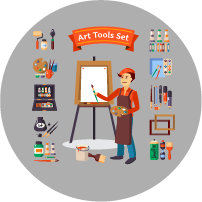
\includegraphics[width=4cm, height=4cm]{Sketch Artists}
  \caption{Digital Board Marker Application: Sketch Artists}
\end{figure}

\bigskip

\subsection{Industrial Presentations}
Digital board marker can be helpful in industrial presentation so that if any person cannot appear at the particular time, that person can watch the recorded (storage efficient) presentation later. So industry will also have less use of its resources.

\bigskip

\begin{figure}[h]
  \centering
  
\includegraphics[width=5cm, height=3cm]{Industry}
  \caption{Digital Board Marker Application: Industrial Presentations}
\end{figure}

\bigskip













